\documentclass[tikz,border=8pt]{standalone}
\usetikzlibrary{arrows.meta}
\definecolor{bg}{HTML}{FFFFFF}
\definecolor{emb}{HTML}{FCE4D6}
\definecolor{embedge}{HTML}{C47A3A}
\definecolor{attn}{HTML}{FFE9A8}
\definecolor{attnedge}{HTML}{B8860B}
\definecolor{ffn}{HTML}{CFE8F3}
\definecolor{ffnedge}{HTML}{2A6F97}
\definecolor{norm}{HTML}{E3F2E1}
\definecolor{normedge}{HTML}{2E7D4F}
\definecolor{outp}{HTML}{E8E0F5}
\definecolor{outedge}{HTML}{6A3FA0}
\definecolor{stack}{HTML}{F4F4F6}
\definecolor{stackedge}{HTML}{9AA0A6}
\definecolor{ink}{HTML}{233044}
\definecolor{res}{HTML}{C0392B}
\begin{document}
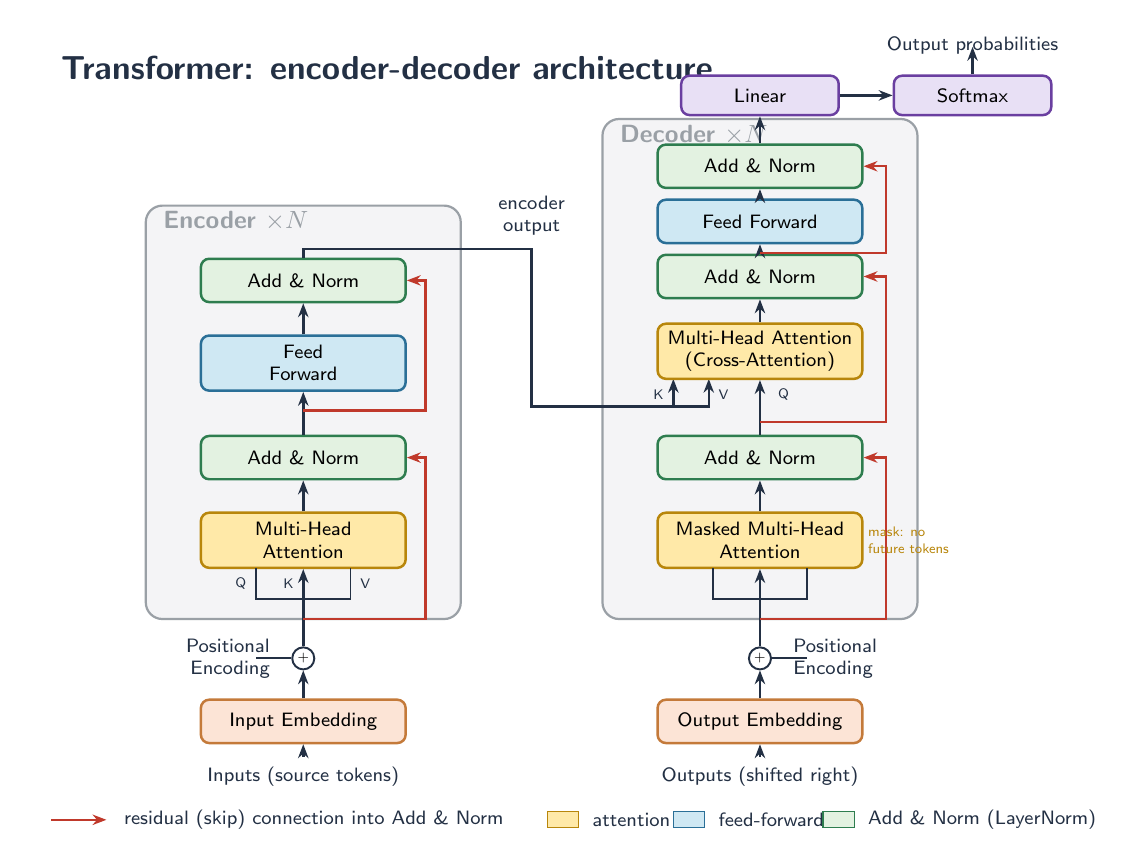
\begin{tikzpicture}[x=1cm,y=1cm,font=\sffamily\scriptsize,
  blk/.style={draw,line width=0.9pt,rounded corners=3pt,align=center,inner sep=0pt,minimum width=2.6cm,minimum height=0.55cm},
  flow/.style={-{Stealth[length=5pt]},line width=0.9pt,ink},
  resid/.style={-{Stealth[length=5pt]},line width=0.9pt,res},
  plus/.style={circle,draw=ink,fill=white,line width=0.7pt,inner sep=0pt,minimum size=0.28cm,font=\sffamily\tiny}]
  \fill[bg] (-0.6,-1.5) rectangle (12.2,8.8);
  \node[font=\sffamily\bfseries\large,text=ink,anchor=west] at (-0.3,8.3) {Transformer: encoder-decoder architecture};

  % ===== stacks =====
  \fill[stack,rounded corners=6pt] (0.9,1.3) rectangle (4.9,6.55);
  \draw[stackedge,line width=0.8pt,rounded corners=6pt] (0.9,1.3) rectangle (4.9,6.55);
  \node[font=\sffamily\bfseries\small,text=stackedge,anchor=west] at (1.0,6.35) {Encoder $\times N$};
  \fill[stack,rounded corners=6pt] (6.7,1.3) rectangle (10.7,7.65);
  \draw[stackedge,line width=0.8pt,rounded corners=6pt] (6.7,1.3) rectangle (10.7,7.65);
  \node[font=\sffamily\bfseries\small,text=stackedge,anchor=west] at (6.8,7.45) {Decoder $\times N$};

  % ===== encoder column (x = 2.9) =====
  \node[blk,draw=embedge,fill=emb] (ie) at (2.9,0.0) {Input Embedding};
  \node[plus] (pe1) at (2.9,0.8) {+};
  \node[font=\sffamily\scriptsize,text=ink,anchor=east,align=right] at (2.6,0.8) {Positional\\Encoding};
  \draw[ink,line width=0.7pt] (2.75,0.8) -- (2.3,0.8);
  \node[blk,draw=attnedge,fill=attn,minimum height=0.7cm] (mha) at (2.9,2.3) {Multi-Head\\Attention};
  \node[blk,draw=normedge,fill=norm] (an1) at (2.9,3.35) {Add \& Norm};
  \node[blk,draw=ffnedge,fill=ffn,minimum height=0.7cm] (ff1) at (2.9,4.55) {Feed\\Forward};
  \node[blk,draw=normedge,fill=norm] (an2) at (2.9,5.6) {Add \& Norm};
  \node[font=\sffamily\scriptsize,text=ink,anchor=north] at (2.9,-0.45) {Inputs (source tokens)};

  \draw[flow] (2.9,-0.45) -- (ie.south);
  \draw[flow] (ie.north) -- (pe1.south);
  \draw[flow] (pe1.north) -- (mha.south);
  % Q,K,V fan-in
  \draw[ink,line width=0.7pt] (2.9,1.55) -- (2.3,1.55) -- (2.3,1.95) (2.9,1.55) -- (3.5,1.55) -- (3.5,1.95);
  \node[font=\sffamily\tiny,text=ink] at (2.3,1.75) [left] {Q};
  \node[font=\sffamily\tiny,text=ink] at (2.9,1.75) [left] {K};
  \node[font=\sffamily\tiny,text=ink] at (3.5,1.75) [right] {V};
  \draw[flow] (mha.north) -- (an1.south);
  \draw[flow] (an1.north) -- (ff1.south);
  \draw[flow] (ff1.north) -- (an2.south);
  % residual connections (red, bypass on the right)
  \draw[resid] (2.9,1.3) -- (4.45,1.3) -- (4.45,3.35) -- (an1.east);
  \draw[resid] (2.9,3.95) -- (4.45,3.95) -- (4.45,5.6) -- (an2.east);
  % encoder output to decoder cross-attention (K, V)
  \draw[flow] (an2.north) -- (2.9,6.0) -- (5.8,6.0) -- (5.8,4.0) -- (7.6,4.0) -- (7.6,4.35);
  \draw[flow] (5.8,4.0) -- (8.05,4.0) -- (8.05,4.35);
  \node[font=\sffamily\scriptsize,text=ink,anchor=south,align=center] at (5.8,6.05) {encoder\\output};
  \node[font=\sffamily\tiny,text=ink] at (7.6,4.15) [left] {K};
  \node[font=\sffamily\tiny,text=ink] at (8.05,4.15) [right] {V};

  % ===== decoder column (x = 8.7) =====
  \node[blk,draw=embedge,fill=emb] (oe) at (8.7,0.0) {Output Embedding};
  \node[plus] (pe2) at (8.7,0.8) {+};
  \node[font=\sffamily\scriptsize,text=ink,anchor=west,align=left] at (9.0,0.8) {Positional\\Encoding};
  \draw[ink,line width=0.7pt] (8.85,0.8) -- (9.3,0.8);
  \node[blk,draw=attnedge,fill=attn,minimum height=0.7cm] (mmha) at (8.7,2.3) {Masked Multi-Head\\Attention};
  \node[blk,draw=normedge,fill=norm] (dn1) at (8.7,3.35) {Add \& Norm};
  \node[blk,draw=attnedge,fill=attn,minimum height=0.7cm] (cross) at (8.7,4.7) {Multi-Head Attention\\(Cross-Attention)};
  \node[blk,draw=normedge,fill=norm] (dn2) at (8.7,5.65) {Add \& Norm};
  \node[blk,draw=ffnedge,fill=ffn,minimum height=0.55cm] (ff2) at (8.7,6.35) {Feed Forward};
  \node[blk,draw=normedge,fill=norm] (dn3) at (8.7,7.05) {Add \& Norm};
  \node[font=\sffamily\scriptsize,text=ink,anchor=north,align=center] at (8.7,-0.45) {Outputs (shifted right)};

  \draw[flow] (8.7,-0.45) -- (oe.south);
  \draw[flow] (oe.north) -- (pe2.south);
  \draw[flow] (pe2.north) -- (mmha.south);
  \draw[ink,line width=0.7pt] (8.7,1.55) -- (8.1,1.55) -- (8.1,1.95) (8.7,1.55) -- (9.3,1.55) -- (9.3,1.95);
  \draw[flow] (mmha.north) -- (dn1.south);
  \draw[flow] (dn1.north) -- (cross.south);   % Q from decoder
  \node[font=\sffamily\tiny,text=ink] at (8.7,4.15) [right=3pt] {Q};
  \draw[flow] (cross.north) -- (dn2.south);
  \draw[flow] (dn2.north) -- (ff2.south);
  \draw[flow] (ff2.north) -- (dn3.south);
  % decoder residuals
  \draw[resid] (8.7,1.3) -- (10.3,1.3) -- (10.3,3.35) -- (dn1.east);
  \draw[resid] (8.7,3.8) -- (10.3,3.8) -- (10.3,5.65) -- (dn2.east);
  \draw[resid] (8.7,5.95) -- (10.3,5.95) -- (10.3,7.05) -- (dn3.east);
  % mask note
  \node[font=\sffamily\tiny,text=attnedge,anchor=west,align=left] at (9.95,2.3) {mask: no\\future tokens};

  % ===== output head =====
  \node[blk,draw=outedge,fill=outp,minimum width=2.0cm,minimum height=0.5cm] (lin) at (8.7,7.95) {Linear};
  \node[blk,draw=outedge,fill=outp,minimum width=2.0cm,minimum height=0.5cm] (sm) at (11.4,7.95) {Softmax};
  \draw[flow] (dn3.north) -- (lin.south);
  \draw[flow] (lin.east) -- (sm.west);
  \draw[flow] (sm.north) -- ++(0,0.35);
  \node[font=\sffamily\scriptsize,text=ink,anchor=south] at (11.4,8.35) {Output probabilities};

  % ===== legend =====
  \draw[resid] (-0.3,-1.25) -- (0.4,-1.25); \node[anchor=west,text=ink] at (0.5,-1.25) {residual (skip) connection into Add \& Norm};
  \fill[attn,draw=attnedge] (6.0,-1.35) rectangle (6.4,-1.15); \node[anchor=west,text=ink] at (6.45,-1.25) {attention};
  \fill[ffn,draw=ffnedge] (7.6,-1.35) rectangle (8.0,-1.15); \node[anchor=west,text=ink] at (8.05,-1.25) {feed-forward};
  \fill[norm,draw=normedge] (9.5,-1.35) rectangle (9.9,-1.15); \node[anchor=west,text=ink] at (9.95,-1.25) {Add \& Norm (LayerNorm)};
\end{tikzpicture}
\end{document}
